\begin{soln}
	Consider the instance:

	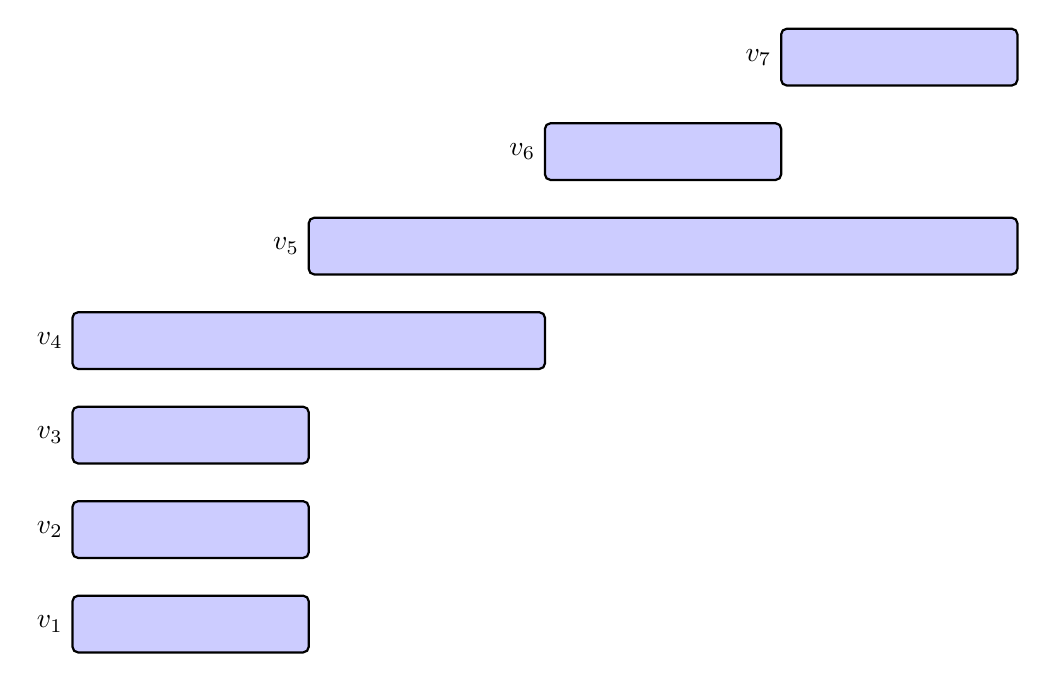
\begin{tikzpicture}[xscale=3, yscale=1.2]

		% Draw each interval as a bar
		\foreach \name/\start/\end/\y in {
				v_1/0/1/1,
				v_2/0/1/2,
				v_3/0/1/3,
				v_4/0/2/4,
				v_5/1/4/5,
				v_6/2/3/6,
				v_7/3/4/7
			} {
				\draw[thick, fill=blue!20, rounded corners=2pt] (\start,\y) rectangle (\end,\y+0.6);
				\node[left] at (\start,\y+0.3) {\(\name\)};
			}

	\end{tikzpicture}


	We see that in the proposed greedy algorithm that \(v_4\) intersects with the most amount of shifts, \(4\).

	After removing all intersections, only \(v_6, v_7\) remains, since those two are disjoint, the greedy algorithm returns volunteers \(v_4, v_6, v_7\) as its best solution.

	But notice that, by taking volunteers the two \(v_1, v_5\) we sufficiently cover all shifts in the set, thus this greedy algorithm is not optimal on all instances.

\end{soln}
